\section{Use Cases}

\subsection{Use Case Diagram}
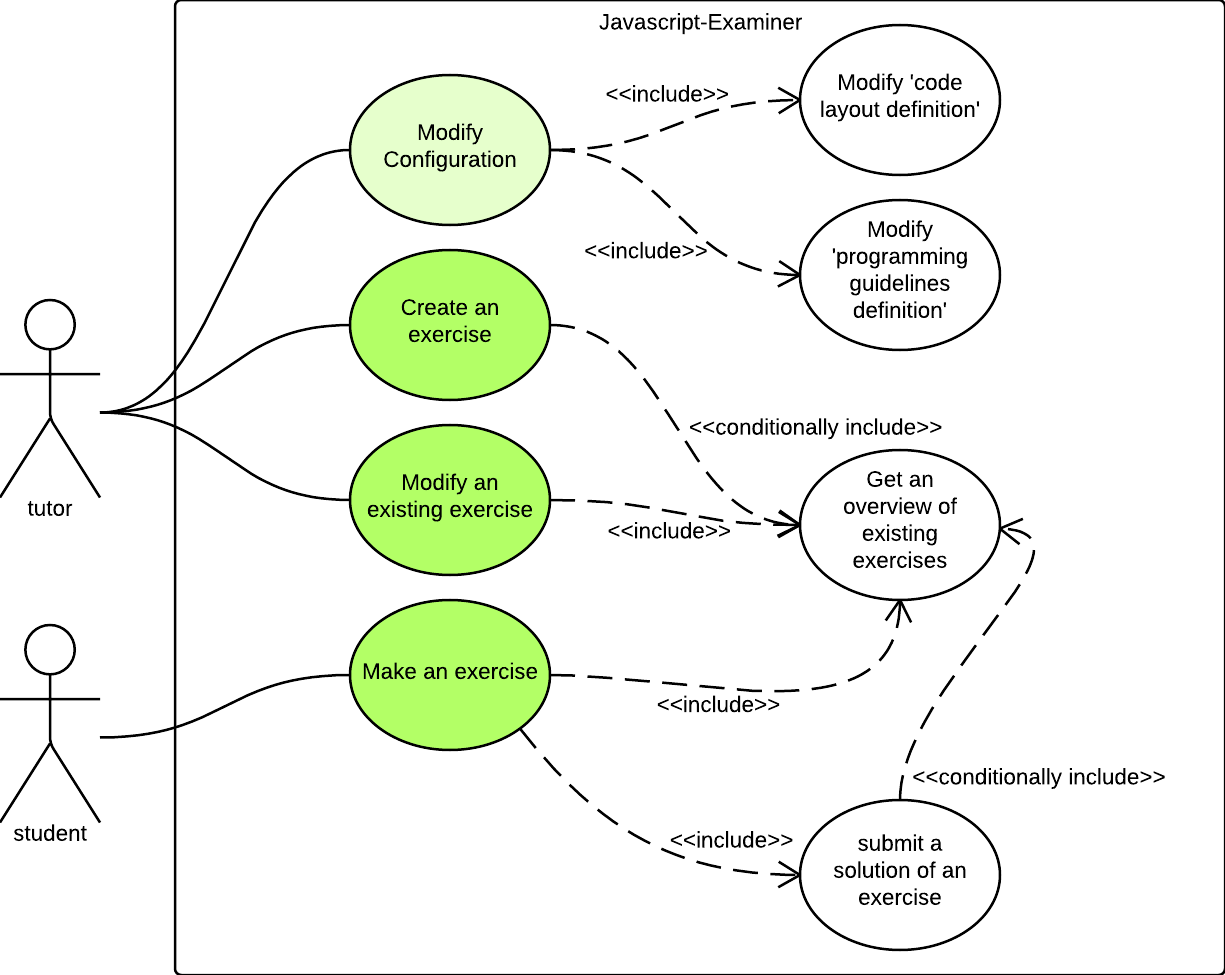
\includegraphics[scale=1]{appendices/diagrams-images/use-case-diagram}

\subsection{Main Use Cases}

\subsubsection{Create an Exercise}
\begin{mdframed} [rightmargin=-100pt]
\begin{description}
  \item[Scope] JavaScript-examiner
  \item[Level] user goal
  \item[Primary Actor] Tutor
  \item[Preconditions] -
  \item[Success Guarantee] The tutor has created an exercise.
  \item[Main Success Scenario] \mbox{}
	\begin{enumerate}
	  \item Tutor starts creation of a new exercise.
	  \item System requests general exercise information.
	  \item Tutor provides general exercise information.
    \item System request model solution(s).
    \item Tutor provides model solution(s).
    \item System requests test suite.
    \item Tutor provides test suite.
    \item System shows overview with exercise information.
    \item Tutor acknowledges exercise information.
    \item System confirms the exercise is successfully added.
	\end{enumerate}
\end{description}
\end{mdframed}

\subsubsection{Modify an Exercise}
\begin{mdframed} [rightmargin=-100pt]
\begin{description}
  \item[Scope] JavaScript-examiner
  \item[Level] user goal
  \item[Primary Actor] Tutor
  \item[Preconditions] There is at least 1 exercise available.
  \item[Success Guarantee] The tutor has modified an exercise.
  \item[Main Success Scenario] \mbox{}
	\begin{enumerate}
	  \item Tutor selects exercise from overview. \underline{Include: get
        an overview of available exercises}
	  \item System presents editable overview with exercise specifics.
	  \item Tutor modifies exercise.
    \item Tutor submits modified exercise.
    \item System confirms the exercise is successfully modified.
	\end{enumerate}
\end{description}
\end{mdframed}

\subsubsection{Make an exercise}
\begin{mdframed} [rightmargin=-100pt]
\begin{description}
  \item[Scope] JavaScript-examiner
  \item[Level] user goal
  \item[Primary Actor] Student
  \item[Preconditions] There is at least 1 exercise available.
  \item[Success Guarantee] Student has received feedback on the submitted 
	solution.
  \item[Main Success Scenario] \mbox{}
	\begin{enumerate}
	  \item Student selects exercise from overview. \underline{Include: get
        an overview of available exercises}
	  \item Student requests exercise instruction.
	  \item System presents exercise instruction.
	  \item Student submits solution. \underline{Include: submit a solution of 
	    an exercise}
	  \item System presents feedback
	\end{enumerate}
\end{description}
\end{mdframed}

\newpage
\subsection{Supporting Use Cases}

\subsubsection{Get an overview of existing exercises}
\begin{mdframed} [rightmargin=-100pt]
\begin{description}
  \item[Scope] JavaScript-examiner
  \item[Level] Subfunction
  \item[Primary Actor] Student, Tutor
  \item[Preconditions] Usecase \underline{make an exercise}, 
							   \underline{create an exercise} or
							   \underline{modify an exercise} initiated.
  \item[Success Guarantee] An overview of available exercises is 
    presented.
  \item[Main Success Scenario] \mbox{}
    \begin{enumerate} 
	  \item Student / Tutor requests overview of exercises
	  \item System presents overview of exercises
	\end{enumerate}
  \item[(Possible future) Extensions] \mbox{}
    \begin{enumerate}
	  \renewcommand{\labelenumi}{\theenumi a.}
	  \item Only a selection of the exercises is being requested:
		\begin{enumerate}[(1)]
		  \renewcommand{\labelenumii}{\theenumii .}
		  \item Student/Tutor provides a search string.
		  \item System presents the selection of exercises.
		\end{enumerate}
	\end{enumerate}
\end{description}
\end{mdframed}

\subsubsection{Submit the solution of an exercise}
\begin{mdframed} [rightmargin=-100pt]
\begin{description}
  \item[Scope] JavaScript-examiner
  \item[Level] Subfunction
  \item[Primary Actor] Student
  \item[Preconditions] Usecase \underline{make an exercise} initiated.
  \item[Success Guarantee] The solution has been submitted, the student has been
    provided with feedback.
  \item[Main Success Scenario] \mbox{}
    \begin{enumerate}
		\item Student requests submission of the solution.
		\item System requests the solution.
		\item Student submits the solution.
		\item System presents feedback on solution.
    \end{enumerate} 
  \item[Extensions] \mbox{}
	\begin{enumerate}
      \renewcommand{\labelenumi}{\theenumi a.}
	  \item The interaction with the system has been interrupted:
		\begin{enumerate}[(1)]
		  \renewcommand{\labelenumii}{\theenumii .}
		  \item Student selects corresponding exercise from overview. \\
		    \underline{Include: get an overview of available exercises}
		  \item System shows options for selected exercise.
		  \item Student requests submission of the solution.
		\end{enumerate}
	\end{enumerate}
\end{description}
\end{mdframed}